\section{Sammanfattning av energiflöden: energibalanser}
\label{resultsfreerunning}

Genom att summera alla opåverkbara energiflöden fås ett värde på hur mycket energi som behöver tillföras för att uppnå önskad inomhustemperatur. De olika energiflödena är alltså från fasta energikällor, flöde genom väggarna, burspråk och 
tak, genom grunden, av solinstrålning in och strålning ut genom fönstren samt från ofrivillig 
ventilation. Den sista punkten, som orsakas av vind, är satt till noll i april, medan vinden i december är satt till $\unit[7]{m~s^{-1}}$. Denna förlust är inräknad i energiflödet genom respektive fasaddel.

Från fasta energikällor fås alltid ett bidrag på totalt $\unit[10,5]{kW}$, se avsnitt~\ref{sec:constsources}. Ur figurerna i avsnitt~\ref{sec:steadystatewall} får vi energiflödena per kvadratmeter genom de 
olika avsnitten av klimatskalet och med hjälp av areorna i tabell \ref{tbl:uvalue} fås det totala 
energiutflödet genom husets hela klimatskal. Flödet genom grunden beskrivs av figur~\ref{fig:cooling_ground} och solinstrålningen genom fönster
 en solig dag beskrivs av figur~\ref{fig:effekt0415and1231}. Strålningen ut genom fönstren beräknas 
 som svartkroppsstrålning med en transmissionskoefficient i fönstret på 0.9.

Alla dessa energiflöden har sammanfattats i figur~\ref{fig:energyflow_sum} för våra fyra olika 
fall – molnigt respektive soligt aprildygn och  molnigt respektive soligt decemberdygn. Här visas 
summan av de positiva respektive de negativa flödena på grafens positiva respektive 
negativa axel. Den heldragna linjen visar gränsen mellan in- och utflödena. Dessa summeras sedan och visas med en streckad svart linje. Det översta röda 
området som syns tydligt på december-bilderna, figur~\ref{fig:sum_decnosun} och \ref
{fig:sum_decsun}, visar hur mycket större energiutflödet blir när man, som idag, inte har isolerat söder- och västväggarna. Om man isolerar summeras det positiva energiflödet istället upp till och med den orangea linjen. Den summerande svarta linjen visar summan av energiflöden idag, utan isolering på syd- och västväggarna. Flödet genom fönster summerar solinstrålning, långvågig svartkroppsstrålning från rummet och från omgivningen samt konvektion.


\begin{figure}[hpbt]
\centering
\subfloat[\label{fig:sum_aprnosun} Molnigt dygn i april.]{
	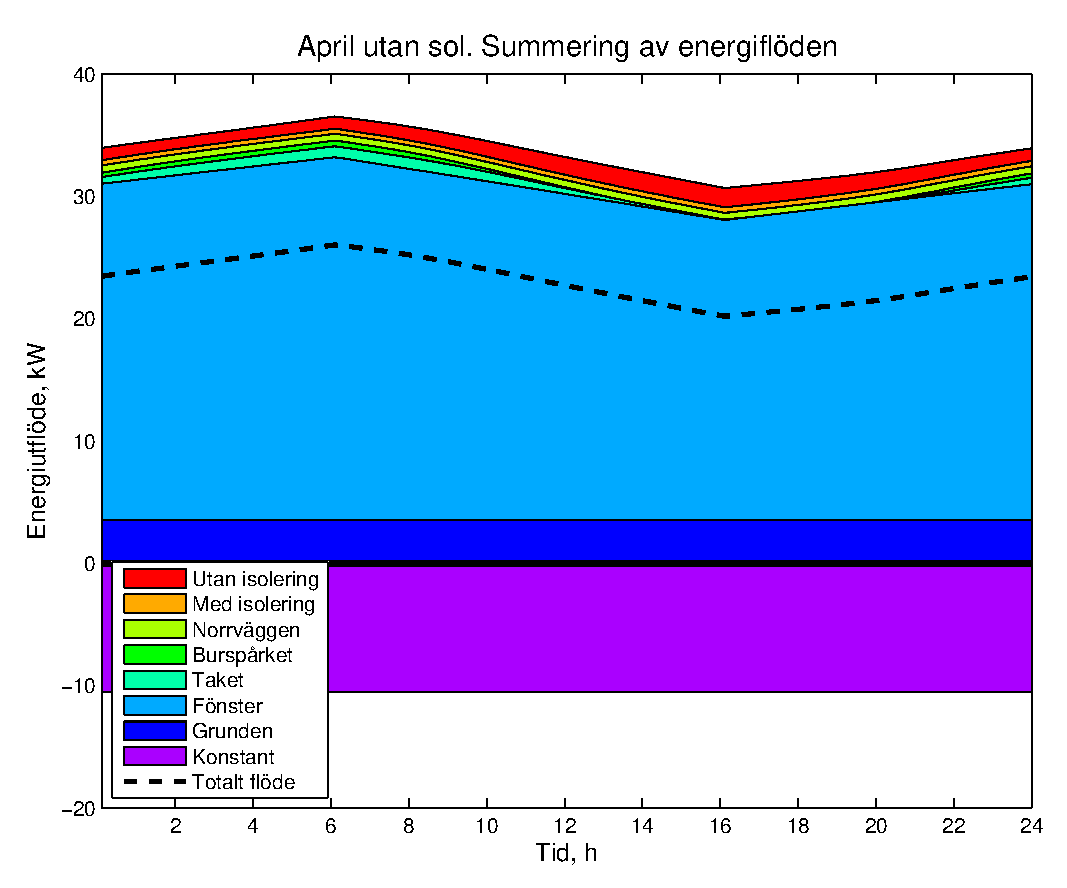
\includegraphics[width=0.5\textwidth]{images/aprnosun_sum.eps}
}
\subfloat[\label{fig:sum_aprsun} Klart dygn i april]{
	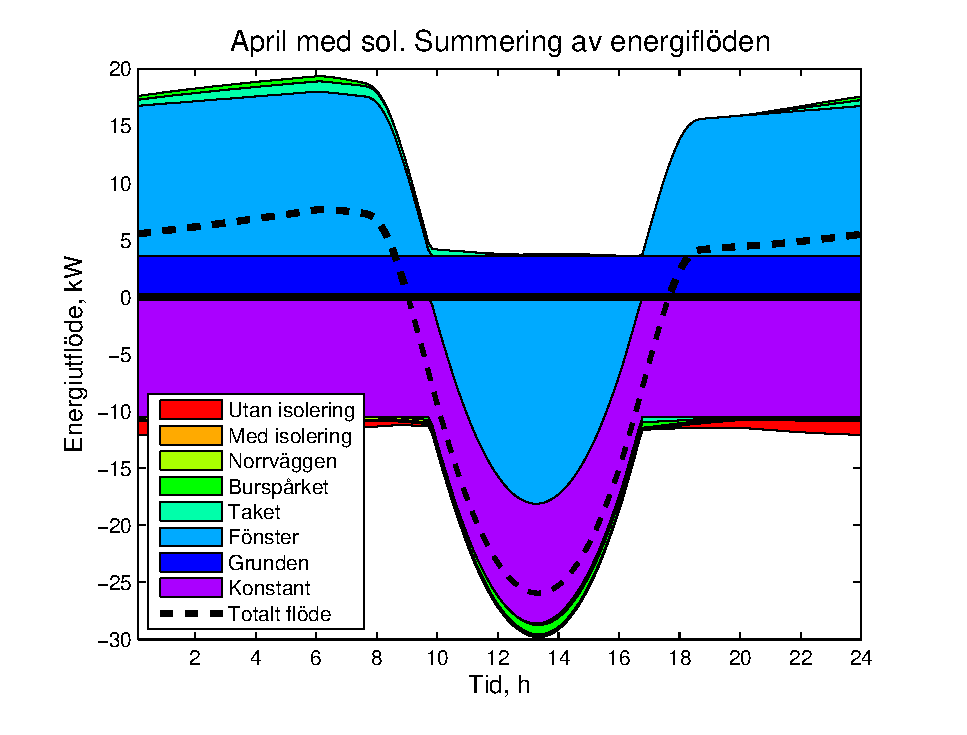
\includegraphics[width=0.5\textwidth]{images/aprsun_sum.eps}
}

\subfloat[\label{fig:sum_decnosun} Molnigt dygn i december.]{
	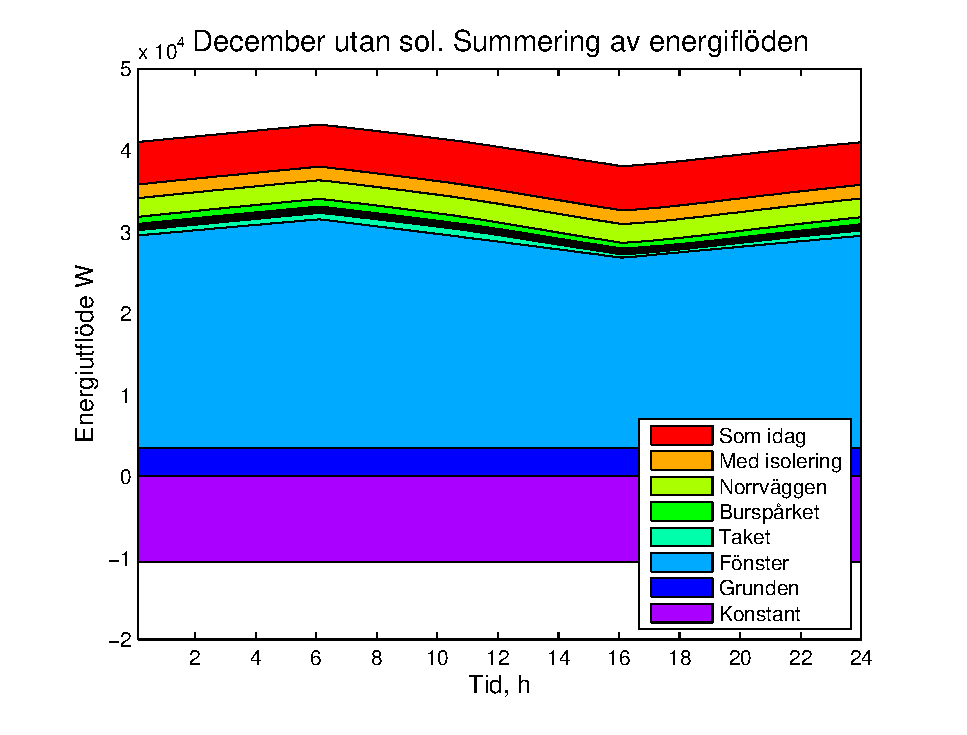
\includegraphics[width=0.5\textwidth]{images/decnosun_sum.eps}
}
\subfloat[\label{fig:sum_decsun} Klart dygn i december.]{
	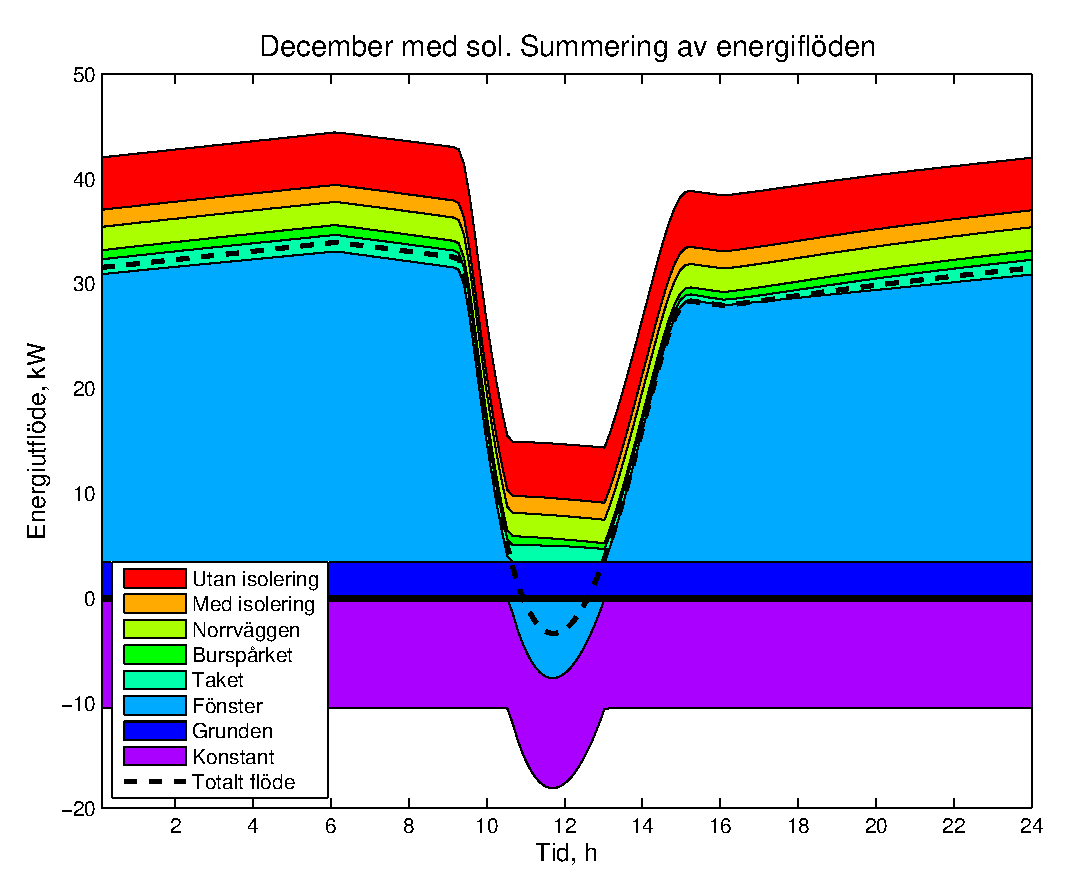
\includegraphics[width=0.5\textwidth]{images/decsun_sum.eps}
}

\caption{\label{fig:energyflow_sum} Totala energiflöden genom byggnaden, där utflöden
 betecknas positivt, och inflöden negativt. Den streckade linjen markerar summering av 
 positiva och negativa energiflöden. Den heldragna något bredare linjen är gränsen mellan in- och utflöden.}
\end{figure}

Det mest framträdande i bilderna är solens påverkan. Det syns också tydligt att fönstren läcker väldigt mycket energi. Under ett klart aprildygn är det genom fönstren som den mesta energin 
kommer in när solen skiner samtidigt som fönstren är den största energitjuven under 
resten av dygnet. Vi ser också att tilläggsisolering av syd-
 och västfasaderna knappast lönar sig en solig dag i april, det gör det däremot i december. Fönstren är dock den enskilt största 
 källan till energiläckage. Genom att jämföra energiflödena under ett soligt dygn i december med ett molnigt konstateras att energiflödet kan minskas med 22\% genom att ta hänsyn till solen, se avsnitt~\ref{subsec:sunhours}.

Vid vind fås ytterligare energiförluster. Med en vindmätare fås vindhastigheten enkelt i varje ögonblick och energiförlusten beräknas enligt avsnitt~\ref{sec:leakagewall} och adderas till befintligt energiflöde. Där kan ses att energiläckaget på grund av infiltrationsförluster vid vind kan bli mycket stora. För att veta exakt hur fastigheten reagerar på vind behöver dock ett trycktest göras.